%# -*- coding:utf-8 -*-
\chapter[基于张量优化的无监督特征选择:CPUFS与CPUFSnn方法]{基于张量优化的无监督特征选择:\\CPUFS与CPUFSnn方法}\label{chap:cpufs}
\echapter{Tensor Optimization-Based Unsupervised Feature Selection: The CPUFS and CPUFSnn Methods}

本章将介绍基于张量优化的无监督特征选择方法——CPUFS与CPUFSnn。首先介绍CPUFS方法的优化模型、优化算法以及关于优化算法的理论收敛性分析与计算复杂度分析。然后在CPUFS方法的基础上直接给出CPUFSnn方法的优化模型,并基于CPUFS方法的优化方法及其理论分析结果直接给出CPUFSnn方法的优化方法及相应的理论分析结果。CPUFS方法的流程如\reffig{fig:CPUFS-routine}所示。

% \section{基于张量优化的无监督特征选择的流程}
% \esection{Workflow of Tensor Optimization-Based Unsupervised Feature Selection}

\begin{figure}[!ht]
	\centering
    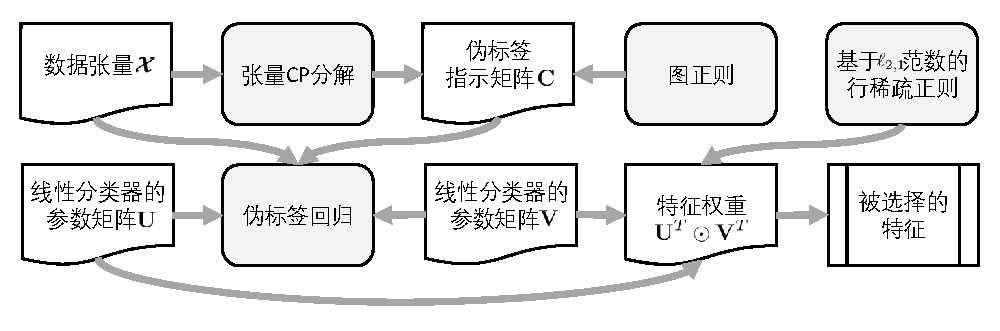
\includegraphics[width=\linewidth]{figures/CPUFS_cn.pdf}
	\caption{CPUFS方法的流程示意图}
	\label{fig:CPUFS-routine}
\end{figure}
\vspace{-0.5em}

\section{CPUFS方法的优化模型}
\esection{The Optimization Model of the CPUFS Method}
本节将给出CPUFS方法的优化模型。本节将首先提出全新的面向张量的线性分类器与特征选择矩阵。

\subsection{面向张量的线性分类器设计}\label{sec:design-classf}
\esubsection{Design of Tensor-Oriented Linear Classifier}
为了保留张量的内在结构信息,本文使用张量mode-$n$积来设计面向张量的线性分类器
% \footnote{值得一提的是,另一种常用的张量的乘积——张量收缩积\ucite{bader2006algorithm}并不能被用来设计面向张量的线性分类器。这是由于张量收缩积会破坏张量的结构信息。}
,从而保留张量的内在结构。具体而言,给定三阶张量$\mathbfcal{X}\in\mathbb{R}^{n_{1}\times n_{2}\times n}$,本文很自然地把线性分类器设计为$(\mydiag(\mathbfcal{X}\times_{1}\boldsymbol{U}\times_{2}\boldsymbol{V}))^{\top}\in\mathbb{R}^{n\times c}$,其中$\boldsymbol{U}\in\mathbb{R}^{c\times n_{1}}$和$\boldsymbol{V}\in\mathbb{R}^{c\times n_{2}}$是该线性分类器的两个协同组成部分,而$c$是数据中的潜在类别数。具体而言,对不同的$j=1,2,\ldots,c$,$\boldsymbol{u}_{j:}$和$\boldsymbol{v}_{j:}$协同地且密不可分地通过
\begin{equation*}
    \left[\boldsymbol{u}_{j:}\boldsymbol{X}^{(1)}\boldsymbol{v}_{j:}^{\top},\boldsymbol{u}_{j:}\boldsymbol{X}^{(2)}\boldsymbol{v}_{j:}^{\top}\ldots,\boldsymbol{u}_{j:}\boldsymbol{X}^{(n)}\boldsymbol{v}_{j:}^{\top}\right]^{\top}\in\mathbb{R}^{n},
\end{equation*}
来生成所有样本关于第$j$个类别的聚类伪标签。可以很直观地看到,在这种方式下,张量的内在结构信息被很好地保留了下来。此外,值得一提的是,本文设计的线性分类器的参数量为$\mathcal{O}((n_1+n_2)c)$,而已有方法(如RUFS\ucite{rufs})基于向量化后数据所设计的线性分类器的参数量为$\mathcal{O}(n_1 n_2 c)$。这表明在高维数据环境下,本文设计的线性分类器的参数量远小于已有方法中的线性分类器的参数量!这个特点不仅使得其可以使用更少的存储空间以及进行更快的数值计算,同时还使得其更不容易过拟合。

\subsection{面向张量的特征选择矩阵设计}\label{sec:design-fsmatrix}
\esubsection{Design of Tensor-Oriented Feature Selection Matrix}
特征选择矩阵的设计应满足以下三个要点:
\begin{enumerate}
    \item 特征选择矩阵应依据参数矩阵$\boldsymbol{U}$和$\boldsymbol{V}$来设计;
    \item 特征选择矩阵应能保留张量数据的内在结构信息;
    \item 特征选择矩阵还应能反应每个特征的重要性。
\end{enumerate}
可以看到,设计该特征选择矩阵并非一件易事。本节接下来详细介绍如何解决这个难题。具体来讲,本文独辟蹊径地将特征选择矩阵设计为$(\boldsymbol{U}^{\top}\odot\boldsymbol{V}^{\top})\in\mathbb{R}^{n_{1}n_{2}\times c}$,原因如下。考虑线性分类器的第$(i,j)$个元素
% 设$(\mydiag(\mathbfcal{X}\times_{1}\boldsymbol{U}\times_{2}\boldsymbol{V}))^{\top}$为$\hat{\boldsymbol{C}}$,然后考虑$\hat{\boldsymbol{C}}$的元素$\hat{c}_{ij}$(它的值指示了我们设计的线性分类器是否将第$i$个样本判为第$j$个类别)。$\hat{c}_{ij}$的计算公式如下
% \begin{equation*}
%     \hat{c}_{ij}=\boldsymbol{u}_{j:}\boldsymbol{X}^{(i)}\boldsymbol{v}_{j:}^{\top}=\sum_{h=1}^{n_{1}}\sum_{g=1}^{n_{2}}u_{jh}v_{jg}x_{hgi}.
% \end{equation*}
\begin{equation*}
    \left((\mydiag(\mathbfcal{X}\times_{1}\boldsymbol{U}\times_{2}\boldsymbol{V}))^{\top}\right)_{ij}=\boldsymbol{u}_{j:}\boldsymbol{X}^{(i)}\boldsymbol{v}_{j:}^{\top}=\sum_{h=1}^{n_{1}}\sum_{g=1}^{n_{2}}u_{jh}v_{jg}x_{hgi},
\end{equation*}
其值表明了线性分类器是否将第$i$个样本判为第$j$个类别。在这个表达式中,$x_{hgi}$代表了$\boldsymbol{X}^{(i)}$的第$(h,g)$个特征的数值大小,而$u_{jh}v_{jg}$由于与样本索引$i$无关可以被解释为第$(h,g)$个特征关于第$j$个类别的特征重要性权重。巧合的是,注意到向量$[u_{1h}v_{1g},u_{2h}v_{2g},\ldots,u_{ch}v_{cg}]$恰巧是$(\boldsymbol{U}^{\top}\odot\boldsymbol{V}^{\top})$的第$((h-1)n_{2}+g)$行。此外,这个巧合的对应关系所蕴含的映射
\begin{equation*}
    (h,g)\mapsto (h-1)n_{2}+g:(\mathbb{Z}\cap [1,n_{1}])\times(\mathbb{Z}\cap [1,n_{2}])\rightarrow(\mathbb{Z}\cap [1,n_{1}n_{2}]),
\end{equation*}
显然是双射,即特征选择矩阵$(\boldsymbol{U}^{\top}\odot\boldsymbol{V}^{\top})$的行向量与数据特征之间存在一一对应关系。因此,将特征选择矩阵定义为$(\boldsymbol{U}^{\top}\odot\boldsymbol{V}^{\top})$。

值得一提的是,由于定义的第$(h,g)$个特征关于第$j$个类别的重要性权重$u_{jh}v_{jg}$由$u_{jh}$和$v_{jg}$两部分组成,并且它们分别关联每个数据样本矩阵的第$h$行和第$g$列。那么,对于位于数据样本矩阵的同一行或者同一列上的所有特征,它们之间的特征重要性权重将会产生相互关联。这是本文的方法能够保留张量的结构信息的理论保证。此外,在实验部分的\refsection{sec:visualization}还会展示,这一机制将赋予被选择特征在位置分布上具有显著的空间结构特征。这是已有的无监督特征选择方法所不具备的特点。


\subsection{CPUFS方法的优化模型}\label{sec:opt-model-CPUFS}
\esubsection{The Optimization Model of the CPUFS Method}
至此,所有用于建立CPUFS方法的优化模型的技术工具都已经在前些章节被介绍或设计。本节接下来直接设计CPUFS方法的优化模型,然后逐项解释所设计的优化模型中的每项及每个约束的目的及意义。具体而言,CPUFS方法的优化模型如下
\begin{gather}\label{eq:tensor-based-ufs}
\begin{aligned}
& \underset{\smash[b]{\substack{\mathclap{\boldsymbol{A},\boldsymbol{B},\boldsymbol{C}}\\\mathclap{\boldsymbol{U},\boldsymbol{V},\boldsymbol{Y}}}}}{\min}
& &  \norm{\mathbfcal{X}-\left\llbracket \boldsymbol{A}, \boldsymbol{B}, \boldsymbol{C} \right\rrbracket}_{F}^{2} + \nu\operatorname{Tr}\left(\boldsymbol{C}^{\top}\boldsymbol{L}\boldsymbol{C}\right) \\ \span&& + \alpha\norm{\left(\mydiag\left(\mathbfcal{X}\times_{1}\boldsymbol{U}\times_{2}\boldsymbol{V}\right)\right)^{\top} - \boldsymbol{C}}_{F}^{2} + \beta \norm{\boldsymbol{U}^{\top}\odot\boldsymbol{V}^{\top}}_{2,1}\\
& \text{s.t.}
& & \boldsymbol{A}\in \mathbb{R}_{+}^{n_1 \times c},~\boldsymbol{B}\in \mathbb{R}_{+}^{n_2 \times c},~\boldsymbol{C}\in \mathbb{R}_{+}^{n \times c},~\boldsymbol{C}=\boldsymbol{Y}\left(\boldsymbol{Y}^{\top} \boldsymbol{Y}\right)^{-\frac{1}{2}},~\boldsymbol{Y}\in\{0,1\}^{n\times c},
\end{aligned}
\raisetag{2.33\normalbaselineskip}
\end{gather}
其中$\nu$、$\alpha$和$\beta$是平衡\refopt{eq:tensor-based-ufs}的目标函数中不同项的重要性大小的权重,$c$是数据样本的潜在类别个数,$n$是数据样本的总数量,$\mathbfcal{X}\in\mathbb{R}_{+}^{n_{1}\times n_{2}\times n}$为输入张量,$\boldsymbol{A} \in \mathbb{R}_{+}^{n_{1}\times c}$、$\boldsymbol{B} \in \mathbb{R}_{+}^{n_{2}\times c}$和$\boldsymbol{C} \in \mathbb{R}_{+}^{n\times c}$为非负张量CP分解的因子矩阵,$\boldsymbol{L} \in \mathbb{R}^{n\times n}$为基于\refsection{sec:graphreg}中方法所构建的带权$k$近邻图所对应的拉普拉斯矩阵,而$\boldsymbol{U}\in\mathbb{R}^{c\times n_{1}}$和$\boldsymbol{V}\in\mathbb{R}^{c\times n_{2}}$为线性分类器$\mydiag(\mathbfcal{X}\times_{1}\boldsymbol{U}\times_{2}\boldsymbol{V})$的两个参数矩阵。本节接下来逐项解释\refopt{eq:tensor-based-ufs}中每项及每个约束的目的及意义:
\begin{enumerate}
    \item $\norm{\mathbfcal{X}-\left\llbracket \boldsymbol{A}, \boldsymbol{B}, \boldsymbol{C} \right\rrbracket}_{F}^{2}$(且$\boldsymbol{A}\in \mathbb{R}_{+}^{n_1 \times c}$,$\boldsymbol{B}\in \mathbb{R}_{+}^{n_2 \times c}$,$\boldsymbol{C}\in \mathbb{R}_{+}^{n \times c}$)是张量$\mathbfcal{X}$的非负张量CP分解的目标函数(请参考\refsection{sec:tensor-decomp})。这一项负责通过挖掘张量的内在特性来生成伪标签$\boldsymbol{C}$($\boldsymbol{C}$将会被用于其它子任务),并保留张量$\mathbfcal{X}$中的结构信息。

    \item $\operatorname{Tr}(\boldsymbol{C}^{\top}\boldsymbol{L}\boldsymbol{C})$是图正则的目标函数(请参考\refsection{sec:graphreg})。这一项负责捕获张量样本之间的内在几何结构信息,并驱使着在数据几何结构上相似的样本点具有尽可能相似的伪标签信息。

    \item $\norm{(\mydiag(\mathbfcal{X}\times_{1}\boldsymbol{U}\times_{2}\boldsymbol{V}))^{\top} - \boldsymbol{C}}_{F}^{2}$是线性分类器$\mydiag(\mathbfcal{X}\times_{1}\boldsymbol{U}\times_{2}\boldsymbol{V})$拟合产生的伪标签$\boldsymbol{C}$的目标函数。简单起见,使用Frobenius范数诱导的度量来量化$\mydiag(\mathbfcal{X}\times_{1}\boldsymbol{U}\times_{2}\boldsymbol{V})$与$\boldsymbol{C}$之间的差距。

    \item $\norm{\boldsymbol{U}^{\top}\odot\boldsymbol{V}^{\top}}_{2,1}$是对特征选择矩阵施加行稀疏正则的目标函数。
    这一项迫使特征选择矩阵的行向量变得稀疏。
    由于特征选择矩阵的每一行编码了不同特征的重要性权重,因此若其某一行的$\ell_{2}$范数越小,则与该行所对应的特征对于拟合伪标签$\boldsymbol{C}$起到的作用也就越小,那么该特征也就越不重要。
    % 因此,可以通过比较特征选择矩阵的行$\ell_{2}$范数大小来选择更高质量的特征。
    % After \refopt{eq:tensor-based-ufs} has been well optimized, we can select features according to the $\ell_{2}$-norms of rows of $(\boldsymbol{U}^{\top}\odot\boldsymbol{V}^{\top})$.
    % Thus, we can select discriminative features according to the $\ell_{2}$-norms of rows of $(\boldsymbol{U}^{\top}\odot\boldsymbol{V}^{\top})$.
    % Therefore, minimizing $\norm{\boldsymbol{U}^{\top}\odot\boldsymbol{V}^{\top}}_{2,1}$ has the functionality to filter out those less important features.

    \item $\boldsymbol{C}=\boldsymbol{Y}(\boldsymbol{Y}^{\top} \boldsymbol{Y})^{-\frac{1}{2}}$(且$\boldsymbol{Y}\in\{0,1\}^{n\times c}$)是迫使产生的伪标签矩阵$\boldsymbol{C}$成为归一化的类指示矩阵的离散约束。
    此处引入二值矩阵$\boldsymbol{Y}\in\{0,1\}^{n\times c}$来描述数据集$\mathcal{D}_{\text{特征选择}}$中的样本-类簇关系,并定义归一化的类指示矩阵为$\Tilde{\boldsymbol{Y}}=\boldsymbol{Y}(\boldsymbol{Y}^{\top} \boldsymbol{Y})^{-1/2}$,而$\Tilde{\boldsymbol{Y}}$与$\boldsymbol{Y}$相比性质更好\ucite{udfs, ndfs, rufs}(例如注意到$\Tilde{\boldsymbol{Y}}^{\top} \Tilde{\boldsymbol{Y}}\allowbreak=(\boldsymbol{Y}^{\top} \boldsymbol{Y})^{-1/2} \boldsymbol{Y}^{\top} \boldsymbol{Y}(\boldsymbol{Y}^{\top} \boldsymbol{Y})^{-1/2}=\boldsymbol{I}_{c}$)。
    % 约束$\boldsymbol{C}$成为归一化的聚类指示矩阵,从而更贴合实际并具有更好性质。
    % 关于归一化的聚类指示矩阵的定义及其意义
\end{enumerate}

总体来看,在\refopt{eq:tensor-based-ufs}中,目标函数的前两项(即上文的1和2)负责在保留张量局部几何结构及其内在结构信息的同时产生高质量的数据伪标签,而目标函数的后两项(即上文的3、4和5)则负责通过线性分类器拟合数据伪标签并基于此实现特征重要性权重的稀疏化。这两个过程将会在训练过程中相互引导对方,以实现更好的效果。然而,由于\refopt{eq:tensor-based-ufs}的约束项存在离散约束,求解的难度实际上是很大的。为了解决这个问题,需要对该优化问题进行一些必要的松弛和等价变换。下一节将讨论这些策略。

% 为了处理张量,几乎所有现有的无监督特征选择方法都牺牲了张量的结构信息以换取数据处理的简单性。但是,这些信息可能是非常重要的。例如,它们可能能为张量分类提供判别信息。然而,我们提出的CPUFS方法利用非负张量CP分解来生成伪分类标签,并使用新设计的面向张量的线性分类器以及特征选择矩阵来进行伪标签回归以及特征权重稀疏化,从而在整个过程中都保留了张量的数据结构信息。


\section{CPUFS方法的优化算法及其理论分析}
\esection{The Optimization Algorithm for Solving the CPUFS Method with Its Theoretical Analysis}
本节将设计一种求解CPUFS方法的高效优化算法,并对该算法进行理论上的收敛性分析以及计算复杂度分析。
\subsection{CPUFS方法的松弛}
\esubsection{Relaxations for the CPUFS Method}
\refopt{eq:tensor-based-ufs}的难点主要在于涉及离散矩阵的约束$\boldsymbol{C}=\boldsymbol{Y}(\boldsymbol{Y}^{\top} \boldsymbol{Y})^{-\frac{1}{2}}$以及$\boldsymbol{Y}\in\{0,1\}^{n\times c}$。为了解决上述难点,需要将矩阵$\boldsymbol{C}$松弛为连续矩阵。尽管如此,直接松弛$\boldsymbol{C}$为连续矩阵可能会带来严重的后果。比方说,如果直接松弛$\boldsymbol{C}$为连续矩阵而不施加任何约束,那么最优的$\boldsymbol{C}$很有可能会是非常稠密的矩阵,但这降低了其作为数据伪标签指示矩阵的效用性,因为希望每个样本具有清晰的聚类隶属度。注意到,在原有约束中,矩阵$\boldsymbol{C}$还有额外的性质,即$\boldsymbol{C}^{\top}\boldsymbol{C}=\boldsymbol{I}_{c}$。该性质可以帮助摆脱绝大多数不理想的解,原因在于:根据文献\ucite{ding2005equivalence},由于正交约束和非负约束的同时存在,矩阵$\boldsymbol{C}$的每行中都只可能存在一个非零元素,且该元素指示了对应于该行的样本的分类情况。
% 该属性摆脱了非负张量CP分解的因子矩阵的稠密本质,从而为其它组成模组提供更具判别性的伪分类标签。
因此,将\refopt{eq:tensor-based-ufs}松弛为如下优化问题
\begin{equation*}
\begin{aligned}
& \underset{\smash[b]{\substack{\mathclap{\boldsymbol{A},\boldsymbol{B},\boldsymbol{C},}\\\mathclap{\boldsymbol{U},\boldsymbol{V}}}}}{\min}
& &  \norm{\mathbfcal{X}-\left\llbracket \boldsymbol{A}, \boldsymbol{B}, \boldsymbol{C} \right\rrbracket}_{F}^{2} + \nu\operatorname{Tr}\left(\boldsymbol{C}^{\top}\boldsymbol{L}\boldsymbol{C}\right) \\ \span&& + \alpha\norm{\left(\mydiag\left(\mathbfcal{X}\times_{1}\boldsymbol{U}\times_{2}\boldsymbol{V}\right)\right)^{\top} - \boldsymbol{C}}_{F}^{2} + \beta \norm{\boldsymbol{U}^{\top}\odot\boldsymbol{V}^{\top}}_{2,1}\\
& \text{s.t.}
& & \boldsymbol{A}\in \mathbb{R}_{+}^{n_1 \times c},~\boldsymbol{B}\in \mathbb{R}_{+}^{n_2 \times c},~\boldsymbol{C}\in \mathbb{R}_{+}^{n \times c},~\boldsymbol{C}^{\top}\boldsymbol{C} = \boldsymbol{I}_{c}.
\end{aligned}
\end{equation*}
然而,尽管已经做了一些松弛,同时施加在矩阵$\boldsymbol{C}$上的非负约束和正交约束仍然使得目标函数难以优化。受到文献\ucite{socfs}的启发,本节提出了另一个等价的优化问题
\begin{equation*}\label{eq:cpufs-equiv}
    \begin{aligned}
    & \underset{\smash[b]{\substack{\mathclap{\boldsymbol{A},\boldsymbol{B},\boldsymbol{C},}\\\mathclap{\boldsymbol{F},\boldsymbol{U},\boldsymbol{V}}}}}{\min}
    & &  \norm{\mathbfcal{X}-\left\llbracket \boldsymbol{A}, \boldsymbol{B}, \boldsymbol{C} \right\rrbracket}_{F}^{2} + \nu\operatorname{Tr}\left(\boldsymbol{C}^{\top}\boldsymbol{L}\boldsymbol{F}\right) \\ \span&& + \alpha\norm{\left(\mydiag\left(\mathbfcal{X}\times_{1}\boldsymbol{U}\times_{2}\boldsymbol{V}\right)\right)^{\top} - \boldsymbol{F}}_{F}^{2} + \beta \norm{\boldsymbol{U}^{\top}\odot\boldsymbol{V}^{\top}}_{2,1}\\
    & \text{s.t.}
    & & \boldsymbol{A}\in \mathbb{R}_{+}^{n_1 \times c},~\boldsymbol{B}\in \mathbb{R}_{+}^{n_2 \times c},~\boldsymbol{F}\in \mathbb{R}_{+}^{n \times c},~\boldsymbol{F}=\boldsymbol{C},~\boldsymbol{C}^{\top}\boldsymbol{C} = \boldsymbol{I}_{c},
    \end{aligned}
\end{equation*}
其中$\boldsymbol{F}$为辅助矩阵。
% 它旨在
% \begin{enumerate*}[label=(\arabic*)]
%     \item 替矩阵$\boldsymbol{C}$分担之前施加在它上面的非负约束$\boldsymbol{C}\geq 0$,以及
%     \item 将目标函数中的$\operatorname{Tr}(\boldsymbol{C}^{\top}\boldsymbol{L}\boldsymbol{C})$以及$\Vert(\mydiag(\mathbfcal{X}\times_{1}\boldsymbol{U}\times_{2}\boldsymbol{V}))^{\top} - \boldsymbol{C}\Vert_{F}^{2}$分别转化为更容易优化的$\operatorname{Tr}(\boldsymbol{C}^{\top}\boldsymbol{L}\boldsymbol{F})$和$\Vert(\mydiag(\mathbfcal{X}\times_{1}\boldsymbol{U}\times_{2}\boldsymbol{V}))^{\top} - \boldsymbol{F}\Vert_{F}^{2}$。
% \end{enumerate*}
通过定义度量违反约束$\boldsymbol{F}=\boldsymbol{C}$的程度的罚函数$\norm{\boldsymbol{C}-\boldsymbol{F}}_{F}^{2}$,并将该罚函数叠加到目标函数上去,可以将上述优化问题转化为以下更易求解的优化问题
\begin{gather}\label{eq:alterobj}
\begin{aligned}
& \underset{\smash[b]{\substack{\mathclap{\boldsymbol{A},\boldsymbol{B},\boldsymbol{C},}\\\mathclap{\boldsymbol{F},\boldsymbol{U},\boldsymbol{V}}}}}{\min}
& &  \norm{\mathbfcal{X}-\left\llbracket \boldsymbol{A}, \boldsymbol{B}, \boldsymbol{C} \right\rrbracket}_{F}^{2} + \nu\operatorname{Tr}\left(\boldsymbol{C}^{\top}\boldsymbol{L}\boldsymbol{F}\right) + \eta\norm{\boldsymbol{C}-\boldsymbol{F}}_{F}^{2} \\ \span&& + \alpha\norm{\left(\mydiag\left(\mathbfcal{X}\times_{1}\boldsymbol{U}\times_{2}\boldsymbol{V}\right)\right)^{\top} - \boldsymbol{F}}_{F}^{2} + \beta \norm{\boldsymbol{U}^{\top}\odot\boldsymbol{V}^{\top}}_{2,1}\\
& \text{s.t.}
& & \boldsymbol{A}\in \mathbb{R}_{+}^{n_1 \times c},~\boldsymbol{B}\in \mathbb{R}_{+}^{n_2 \times c},~\boldsymbol{F}\in \mathbb{R}_{+}^{n \times c},~\boldsymbol{C}^{\top}\boldsymbol{C} = \boldsymbol{I}_{c},
\end{aligned}
\end{gather}
其中$\eta$是足够大的常数,用以保证$\boldsymbol{F}$和$\boldsymbol{C}$在数值上足够接近。
至此,CPUFS方法的优化难度已经被大大降低,即现在每个优化变量只有至多一个约束。
% 然而,尽管CPUFS方法已经得到松弛,
% 尽管如此,由于\refopt{eq:alterobj}仍然为非常复杂的优化问题,因而不可能直接找到它的全局最优解。
尽管如此,仍然不可能直接找到\refopt{eq:alterobj}的全局最优解。
因此,下一节将基于迭代优化的策略设计一种优化算法用以求解\refopt{eq:alterobj}。

\subsection{优化算法设计}
\esubsection{Design of the Optimization Algorithm}
本节设计一种用于求解\refopt{eq:alterobj}的高效迭代优化算法。本节接下来依次推导各个优化变量的更新公式。

\textbf{$\boldsymbol{A}$的更新:}通过简单的代数运算以及应用\refsection{sec:tensor-decomp}中介绍的mode-$k$展开技巧,仅与$\boldsymbol{A}$有关的子问题即为以下非负矩阵分解问题\ucite{lee2001algorithms}
\begin{equation*}
    \begin{aligned}
    &\underset{\mathclap{\boldsymbol{A}}}{\min}\Hquad &&\norm{\boldsymbol{X}_{\left(1\right)}-\boldsymbol{A}\left(\boldsymbol{C}\odot\boldsymbol{B}\right)^{\top}}_{F}^{2}\\
    & \text{s.t.} && \boldsymbol{A}\in \mathbb{R}_{+}^{n_1 \times c},
    \end{aligned}
\end{equation*}
% 而这个问题已经被广泛研究。
则可以应用\refsection{sec:nmf-dec}中介绍的Lee-Seung算法\ucite{lee2001algorithms}来更新之,即
\begin{equation*}
% \label{eq:updateA}
    \boldsymbol{A}\leftarrow\boldsymbol{A}\oast\frac{\boldsymbol{X}_{(1)}\left(\boldsymbol{C}\odot\boldsymbol{B}\right)}{\boldsymbol{A}\left(\boldsymbol{C}\odot\boldsymbol{B}\right)^{\top}\left(\boldsymbol{C}\odot\boldsymbol{B}\right)}.
\end{equation*}

\textbf{$\boldsymbol{B}$的更新:}与$\boldsymbol{A}$子问题类似,仅与$\boldsymbol{B}$有关的子问题也为非负矩阵分解问题,即
\begin{equation*}
    \begin{aligned}
    &\underset{\mathclap{\boldsymbol{B}}}{\min}\Hquad &&\norm{\boldsymbol{X}_{\left(2\right)}-\boldsymbol{B}\left(\boldsymbol{C}\odot\boldsymbol{A}\right)^{\top}}_{F}^{2}\\
    & \text{s.t.} && \boldsymbol{B}\in \mathbb{R}_{+}^{n_2 \times c},
    \end{aligned}
\end{equation*}
则可以再次应用Lee-Seung算法的来更新之,即
\begin{equation*}
% \label{eq:updateB}
    \boldsymbol{B}\leftarrow\boldsymbol{B}\oast\frac{\boldsymbol{X}_{(2)}\left(\boldsymbol{C}\odot\boldsymbol{A}\right)}{\boldsymbol{B}\left(\boldsymbol{C}\odot\boldsymbol{A}\right)^{\top}\left(\boldsymbol{C}\odot\boldsymbol{A}\right)}.
\end{equation*}

\textbf{$\boldsymbol{C}$的更新:}仅与$\boldsymbol{C}$有关的子问题为
\begin{equation*}
    \begin{aligned}
    &\underset{\boldsymbol{C}}{\min} \Hquad &&\norm{\boldsymbol{X}_{\left(3\right)}-\boldsymbol{C}\left(\boldsymbol{B}\odot\boldsymbol{A}\right)^{\top}}_{F}^{2} + \nu\operatorname{Tr}\left(\boldsymbol{C}^{\top}\boldsymbol{L}\boldsymbol{F}\right) + \eta\norm{\boldsymbol{C}-\boldsymbol{F}}_{F}^{2}\\
    & \text{s.t.} && \boldsymbol{C}^{\top}\boldsymbol{C}=\boldsymbol{I}_{c},
    \end{aligned}
\end{equation*}
而这个子问题可以被进一步等价为正交普鲁克问题\ucite{viklands2006algorithms}的特例
\begin{equation*}
    \begin{aligned}
    &\underset{\boldsymbol{C}}{\min} \Hquad &&\norm{\boldsymbol{C} - \left(2\boldsymbol{X}_{(3)}\left(\boldsymbol{B}\odot\boldsymbol{A}\right) - \nu\boldsymbol{L}\boldsymbol{F} + 2\eta\boldsymbol{F}\right)}_{F}^{2}\\
    & \text{s.t.} && \boldsymbol{C}^{\top}\boldsymbol{C}=\boldsymbol{I}_{c}.
    \end{aligned}
\end{equation*}
% 而该问题为正交普鲁克问题\ucite{viklands2006algorithms}的特例。

\begin{lemma}[正交普鲁克问题的解\ucite{viklands2006algorithms}]\kaishu
\label{lemma:quad}
给定矩阵$\boldsymbol{P} \in \mathbb{R}^{n \times m}$和$\boldsymbol{Q} \in \mathbb{R}^{n \times d}$,则优化问题
\begin{equation*}
    \begin{aligned}
&\underset{\mathclap{\Tilde{\boldsymbol{T}}}}{\min} \Hquad&&\left\|\boldsymbol{P}\boldsymbol{\Tilde{T}}-\boldsymbol{Q}\right\|_{F}^{2}\\
&\text{s.t.} && \Tilde{\boldsymbol{T}}\Tilde{\boldsymbol{T}}^{\top} = \boldsymbol{I}_{m},
\end{aligned}
\end{equation*}
有如下解析解
\begin{equation*}
    \Tilde{\boldsymbol{T}}=\boldsymbol{U}\boldsymbol{I}_{m,d}\boldsymbol{V}^{\top},
\end{equation*}
其中$\boldsymbol{U} \in \mathbb{R}^{m \times m}$和$\boldsymbol{V} \in \mathbb{R}^{d \times d}$分别为$\boldsymbol{P}^{\top}\boldsymbol{Q}$的奇异值分解的左右奇异矩阵。
\end{lemma}
\noindent 如果令$\boldsymbol{P}=\boldsymbol{I}_{c}$、$\Tilde{\boldsymbol{T}}=\boldsymbol{C}^{\top}$以及$\boldsymbol{Q}=2(\boldsymbol{B}\odot\boldsymbol{A})^{\top}\boldsymbol{X}_{(3)}^{\top}-\nu\boldsymbol{F}^{\top}\boldsymbol{L}^{\top} + 2\eta\boldsymbol{F}^{\top}$,
% \begin{equation*}
%     \boldsymbol{P}=\boldsymbol{I}_{c},~
%     \Tilde{\boldsymbol{T}}=\boldsymbol{C}^{\top},~\text{以及}~
%     \boldsymbol{Q}=2(\boldsymbol{B}\odot\boldsymbol{A})^{\top}\boldsymbol{X}_{(3)}^{\top}-\nu\boldsymbol{F}^{\top}\boldsymbol{L}^{\top} + 2\eta\boldsymbol{F}^{\top},
% \end{equation*}
那么\reflemma{lemma:quad}中的优化问题将与$\boldsymbol{C}$子问题一致。由此,利用\reflemma{lemma:quad}可以得到$\boldsymbol{C}$子问题的最优更新方式,即
\begin{equation*}
% \label{eq:updateC}
    \boldsymbol{C} \leftarrow \boldsymbol{V}_{\boldsymbol{C}}\boldsymbol{I}_{n,c}\boldsymbol{U}_{\boldsymbol{C}}^{\top},
\end{equation*}
其中$\boldsymbol{U}_{\boldsymbol{C}}$和$\boldsymbol{V}_{\boldsymbol{C}}$分别为$2(\boldsymbol{B}\odot\boldsymbol{A})^{\top}\boldsymbol{X}_{(3)}^{\top}-\nu\boldsymbol{F}^{\top}\boldsymbol{L}^{\top} + 2\eta\boldsymbol{F}^{\top}$的奇异值分解的左右奇异矩阵。

\textbf{$\boldsymbol{F}$的更新:}仅与$\boldsymbol{F}$有关的子问题为
\begin{equation*}
\begin{aligned}
    &\underset{\mathclap{\boldsymbol{F}}}{\min} \Hquad &&\alpha\norm{\left(\mydiag\left(\mathbfcal{X}\times_{1}\boldsymbol{U}\times_{2}\boldsymbol{V}\right)\right)^{\top} - \boldsymbol{F}}_{F}^{2} + \nu\operatorname{Tr}\left(\boldsymbol{C}^{\top}\boldsymbol{L}\boldsymbol{F}\right) + \eta\norm{\boldsymbol{C}-\boldsymbol{F}}_{F}^{2}\\
    & \text{s.t.} && \boldsymbol{F}\in \mathbb{R}_{+}^{n \times c},
\end{aligned}
\end{equation*}
而这个子问题可以被进一步等价为
\begin{equation*}
    \begin{aligned}
    &\underset{\mathclap{\boldsymbol{F}}}{\min} \Hquad &&\norm{\boldsymbol{F}-\frac{\alpha\left(\mydiag\left(\mathbfcal{X}\times_{1}\boldsymbol{U}\times_{2}\boldsymbol{V}\right)\right)^{\top}+\eta\boldsymbol{C} -\frac{\nu}{2}\boldsymbol{L}^{\top}\boldsymbol{C}}{\alpha+\eta} }_{F}^{2}\\
    & \text{s.t.} && \boldsymbol{F}\in \mathbb{R}_{+}^{n \times c},
    \end{aligned}
\end{equation*}
很明显,$\boldsymbol{F}$子问题的最优更新方式为
\begin{equation}
\label{eq:updateF}
    \boldsymbol{F}\leftarrow\frac{1}{\alpha+\eta}\left(\alpha\left(\mydiag\left(\mathbfcal{X}\times_{1}\boldsymbol{U}\times_{2}\boldsymbol{V}\right)\right)^{\top} +\eta\boldsymbol{C}-\frac{\nu}{2}\boldsymbol{L}^{\top}\boldsymbol{C}\right)_{+}.
\end{equation}

\textbf{$\boldsymbol{U}$和$\boldsymbol{V}$的更新:}仅与$\boldsymbol{U}$和$\boldsymbol{V}$有关的子问题为
\begin{equation*}
% \hspace{-1em}
    \underset{\mathclap{\boldsymbol{U},\boldsymbol{V}}}{\min} \quad \alpha\norm{\left(\mydiag\left(\mathbfcal{X}\times_{1}\boldsymbol{U}\times_{2}\boldsymbol{V}\right)\right)^{\top} - \boldsymbol{F}}_{F}^{2} + \beta \norm{\boldsymbol{U}^{\top}\odot\boldsymbol{V}^{\top}}_{2,1}.
\end{equation*}
可以发现,这是无约束的优化问题。该优化问题的目标函数具有一些良好的性质,见下面的定理。
\begin{theorem}\label{thm:UVcvx}\kaishu
    函数
    \begin{equation*}
        \alpha\norm{\left(\mydiag\left(\mathbfcal{X}\times_{1}\boldsymbol{U}\times_{2}\boldsymbol{V}\right)\right)^{\top} - \boldsymbol{F}}_{F}^{2} + \beta \norm{\boldsymbol{U}^{\top}\odot\boldsymbol{V}^{\top}}_{2,1},
    \end{equation*}
    关于矩阵$\boldsymbol{U}$(或$\boldsymbol{V}$)是凸的。
\end{theorem}
\noindent 为了证明这个定理,首先证明以下若干引理。
\begin{lemma}\label{lemma:UVcvx1}\kaishu
    $\norm{(\mydiag(\mathbfcal{X}\times_{1}\boldsymbol{U}\times_{2}\boldsymbol{V}))^{\top} - \boldsymbol{F}}_{F}^{2}$关于矩阵$\boldsymbol{U}$(或$\boldsymbol{V}$)是凸的。
\end{lemma}

\begin{proof}
    显然,$\boldsymbol{U}\mapsto(\mydiag(\mathbfcal{X}\times_{1}\boldsymbol{U}\times_{2}\boldsymbol{V}))^{\top} - \boldsymbol{F}$是矩阵$\boldsymbol{U}$的仿射函数。此外,由于Frobenius范数是一种范数,所以$\norm{\cdot}_{F}^{2}$是凸函数
    % \footnote{这并不是显然的结果。这是由于$\boldsymbol{X}\mapsto\norm{\boldsymbol{X}}_{F}^{2}:\mathbb{R}^{m\times n}\rightarrow\mathbb{R}_{+}$可以看作是凸函数$g(\boldsymbol{X})=\norm{\boldsymbol{X}}_{F}:\mathbb{R}^{m\times n}\rightarrow:\mathbb{R}_{+}$和凸函数$f(x)=x^{2}:\mathbb{R}_{+}\rightarrow\mathbb{R}_{+}$的复合函数$f\circ g$,并且$f(x)$在其定义域上是非递减的,因而由文献\ucite{boyd2004convex}即可得上述断言。}
    。由于凸函数与仿射函数的复合函数仍然是凸函数\ucite{boyd2004convex},那么可以推出$\lVert(\mydiag(\mathbfcal{X}\times_{1}\boldsymbol{U}\times_{2}\boldsymbol{V}))^{\top} \allowbreak - \boldsymbol{F}\rVert_{F}^{2}$关于矩阵$\boldsymbol{U}$是凸的。同样地,也可以推出,$\norm{(\mydiag(\mathbfcal{X}\times_{1}\boldsymbol{U}\times_{2}\boldsymbol{V}))^{\top} - \boldsymbol{F}}_{F}^{2}$关于矩阵$\boldsymbol{V}$也是凸的。
\end{proof}\vspace{0.5em}

% \begin{proof}
%     我们首先证明$\norm{(\mydiag(\mathbfcal{X}\times_{1}\boldsymbol{U}\times_{2}\boldsymbol{V}))^{\top} - \boldsymbol{F}}_{F}^{2}$对矩阵$\boldsymbol{U}$的每一行$\boldsymbol{u}_{i:}$都是凸的。简单的计算表明
%     \begin{equation*}
%         \nabla_{\boldsymbol{u}_{i:}}^{2}\left(\norm{\left(\mydiag\left(\mathbfcal{X}\times_{1}\boldsymbol{U}\times_{2}\boldsymbol{V}\right)\right)^{\top} - \boldsymbol{F}}_{F}^{2}\right) = 2\sum_{k=1}^{n}\boldsymbol{X}^{(k)}\boldsymbol{v}_{i:}^{\top}\boldsymbol{v}_{i:}{\boldsymbol{X}^{(k)}}^{\top}\succeq 0.
%     \end{equation*}
%     因此,我们可以得出以下结论:$\norm{(\mydiag(\mathbfcal{X}\times_{1}\boldsymbol{U}\times_{2}\boldsymbol{V}))^{\top} - \boldsymbol{F}}_{F}^{2}$对矩阵$\boldsymbol{U}$的每一行$\boldsymbol{u}_{i:}$都是凸的。同样地,我们也可以证明$\norm{(\mydiag(\mathbfcal{X}\times_{1}\boldsymbol{U}\times_{2}\boldsymbol{V}))^{\top} - \boldsymbol{F}}_{F}^{2}$对矩阵$\boldsymbol{V}$的每一行$\boldsymbol{v}_{i:}$也都是凸的。我们在此处省略证明,以防赘述。
% \end{proof}\vspace{0.5em}

% \begin{lemma}\kaishu
%     $\norm{(\mydiag(\mathbfcal{X}\times_{1}\boldsymbol{U}\times_{2}\boldsymbol{V}))^{\top} - \boldsymbol{F}}_{F}^{2}$分别关于矩阵$\boldsymbol{U}$或$\boldsymbol{V}$都是凸的。
% \end{lemma}

% \begin{proof}
%     这是由于我们有
%     \begin{equation*}
%     \begin{aligned}
%         &\norm{\left(\mydiag\left(\mathbfcal{X}\times_{1}\left(\lambda\boldsymbol{Z}_{1}+\left(1-\lambda\right)\boldsymbol{Z}_{2}\right)\times_{2}\boldsymbol{V}\right)\right)^{\top} - \boldsymbol{F}}_{F}^{2} \\=& \sum_{i=1}^{c}\norm{\left(\mydiag\left(\mathbfcal{X}\times_{1}\left(\lambda(\boldsymbol{z}_{1})_{i:}+\left(1-\lambda\right)(\boldsymbol{z}_{2})_{i:}\right)\times_{2}\boldsymbol{v}_{i:}\right)\right)^{\top} - \boldsymbol{f}_{i}}_{F}^{2} \\\leq& \sum_{i=1}^{c}\left(\lambda\norm{\left(\mydiag\left(\mathbfcal{X}\times_{1}(\boldsymbol{z}_{1})_{i:}\times_{2}\boldsymbol{v}_{i:}\right)\right)^{\top} - \boldsymbol{f}_{i}}_{F}^{2} + \left(1-\lambda\right)\norm{\left(\mydiag\left(\mathbfcal{X}\times_{1}(\boldsymbol{z}_{2})_{i:}\times_{2}\boldsymbol{v}_{i:}\right)\right)^{\top} - \boldsymbol{f}_{i}}_{F}^{2}\right)\\=& \lambda\norm{\left(\mydiag\left(\mathbfcal{X}\times_{1}\boldsymbol{Z}_{1}\times_{2}\boldsymbol{V}\right)\right)^{\top} - \boldsymbol{F}}_{F}^{2} + \left(1-\lambda\right)\norm{\left(\mydiag\left(\mathbfcal{X}\times_{1}\boldsymbol{Z}_{2}\times_{2}\boldsymbol{V}\right)\right)^{\top} - \boldsymbol{F}}_{F}^{2},
%     \end{aligned}
%     \end{equation*}
%     其中不等号部分使用了\reflemma{lemma:thm0}。依据凸函数的定义\ucite{boyd2004convex},$\boldsymbol{U}$部分的证明就完成了。同样的证明方法也可应用在$\boldsymbol{V}$上。为了避免冗余,我们不再赘述。
% \end{proof}\vspace{0.5em}

\begin{lemma}\kaishu
    $\boldsymbol{X}\mapsto\norm{\boldsymbol{X}}_{2,1}:\mathbb{R}^{m\times n}\rightarrow\mathbb{R}_{+}$是关于$\boldsymbol{X}$的凸函数。
\end{lemma}

\begin{proof}
    由于所有的范数都是凸的\ucite{boyd2004convex},因此只需要证明$\ell_{2,1}$范数的确是一种范数即可
%     \footnote{尽管从名字上来看,$\ell_{2,1}$范数似乎就是一种范数,但其实这是需要证明的。例如,$\forall~0\leq p < 1$,虽然都称$\ell_{p}$范数为“范数”,但其实它们并不满足范数的条件。简单的反证法表明,如果它们满足范数的条件,那么它们的下水平集都是凸集。考虑赋范空间$(\mathbb{R}^{d},\norm{\cdot}_{p})$中的单位圆盘$\mathbb{B}_{p}(0,1):=\{\boldsymbol{x}\in\mathbb{R}^{d}\mid\norm{x}_{p}\leq 1\}$,则$\mathbb{B}_{p}(0,1)$为$\ell_{p}$范数的一个下水平集。但由下图所展示的$\{(\mathbb{R}^{2},\norm{\cdot}_{p})\}_{p=1,2,\infty,1/2}$中的单位圆盘(或凭经验)即可得知当$d=2$时,$\forall~0\leq p < 1$,$\mathbb{B}_{p}(0,1)$显然均非凸集。因此$\forall~0\leq p < 1$,$\ell_{p}$范数均不是范数。
%     \begin{center}
%     \resizebox{.8\linewidth}{!}{\begin{tikzpicture}[>=Stealth]
%   \foreach \i in {0,...,3}{
%      \begin{scope}[xshift=\i*3.5cm]
%       \draw [->] (-1.5,0)--(1.5,0);
%       \draw [->] (0,-1.5)--(0,1.5);
%     \end{scope}
%   }
%   \begin{scope}[draw=black]
%      \draw [pattern={Lines[angle=-45,distance=4pt]}] (-1,0)--(0,1)--(1,0)--(0,-1)--cycle;
%      \draw [pattern={Lines[angle=-45,distance=4pt]}](3.5,0) circle (0.88cm);
%      \draw [pattern={Lines[angle=-45,distance=4pt]},xshift=7cm] (-.66,-.66) rectangle (.66,.66);
%      \begin{scope}[xshift=10.5cm]
%       \draw [domain=0:90,samples=100,smooth,variable=\t] plot({-1*cos(\t)^(3)},{1*sin(\t)^(3)});
%       \draw [domain=0:90,samples=100,smooth,variable=\t] plot({-1*cos(\t)^(3)},{-1*sin(\t)^(3)});
%       \draw [domain=0:90,samples=100,smooth,variable=\t] plot({1*cos(\t)^(3)},{-1*sin(\t)^(3)});
%       \draw [domain=0:90,samples=100,smooth,variable=\t] plot({1*cos(\t)^(3)},{1*sin(\t)^(3)});
%      \end{scope}
%      \draw[pattern={Lines[angle=-45,distance=4pt]},xshift=10.5cm] plot[smooth, samples=100, domain=0:90,variable=\t] ({-1*cos(\t)^(3)},{1*sin(\t)^(3)}) -| (0,0) -- cycle;
%      \draw[pattern={Lines[angle=-45,distance=4pt]},xshift=10.5cm] plot[smooth, samples=100, domain=0:90,variable=\t] ({-1*cos(\t)^(3)},{-1*sin(\t)^(3)}) -| (0,0) -- cycle;
%      \draw[pattern={Lines[angle=-45,distance=4pt]},xshift=10.5cm] plot[smooth, samples=100, domain=0:90,variable=\t] ({1*cos(\t)^(3)},{-1*sin(\t)^(3)}) -| (0,0) -- cycle;
%      \draw[pattern={Lines[angle=-45,distance=4pt]},xshift=10.5cm] plot[smooth, samples=100, domain=0:90,variable=\t] ({1*cos(\t)^(3)},{1*sin(\t)^(3)}) -| (0,0) -- cycle;
%   \end{scope}
%   \foreach \i [count=\j from 0] in {1,2,\infty,\frac{1}{2}} \scoped [xshift=\j*3.5cm] { \node [draw=none,anchor=mid west] at (0.25,-1) {$p=\i$}; };
% \end{tikzpicture}}\end{center}}
。简单的计算表明:
    \begin{itemize}
        \item $\norm{\boldsymbol{0}_{m,n}}_{2,1}=0$,
        \item 若$\boldsymbol{X}\in\mathbb{R}^{m\times n}$,则$\norm{\alpha\boldsymbol{X}}_{2,1}=\sum_{j=1}^{m}\norm{\alpha\boldsymbol{x}_{j:}}_{2}=\alpha\sum_{j=1}^{m}\norm{\boldsymbol{x}_{j:}}_{2}=\alpha\norm{\boldsymbol{X}}_{2,1}$,
        \item 若$\boldsymbol{X},\boldsymbol{Y}\in\mathbb{R}^{m\times n}$,则$\norm{\boldsymbol{X}+\boldsymbol{Y}}_{2,1}=\sum_{j=1}^{m}\norm{\boldsymbol{x}_{j:}+\boldsymbol{y}_{j:}}_{2}\leq\sum_{j=1}^{m}\norm{\boldsymbol{x}_{j:}}_{2}+\sum_{j=1}^{m}\norm{\boldsymbol{y}_{j:}}_{2}=\norm{\boldsymbol{X}}_{2,1}+\norm{\boldsymbol{Y}}_{2,1}$,其中不等式的推导使用了$\ell_{2}$范数的三角不等式。
    \end{itemize}
    因此,$\ell_{2,1}$范数的确是一种范数,故$\norm{\boldsymbol{X}}_{2,1}$是关于$\boldsymbol{X}$的凸函数。
\end{proof}\vspace{0.5em}

\begin{lemma}\label{lemma:UVcvx2}\kaishu
    $\norm{\boldsymbol{U}^{\top}\odot\boldsymbol{V}^{\top}}_{2,1}$关于矩阵$\boldsymbol{U}$(或$\boldsymbol{V}$)是凸的。
\end{lemma}

\begin{proof}
    由于
    \begin{equation*}
        \operatorname{vec}\left(\boldsymbol{U}^{\top} \odot \boldsymbol{V}^{\top}\right)=\left(\boldsymbol{I}_{n_{1}c} \odot\left(\boldsymbol{V}^{\top}\left(\boldsymbol{I}_{c} \otimes \boldsymbol{1}^{\top}_{n_{1}}\right)\right)\right)\operatorname{vec}\left(\boldsymbol{U}^{\top}\right),
    \end{equation*}
    因此,$\boldsymbol{U}\mapsto\boldsymbol{U}^{\top}\odot\boldsymbol{V}^{\top}$是矩阵$\boldsymbol{U}$的线性函数。由于凸函数与线性函数的复合函数仍然是凸函数\ucite{boyd2004convex},那么可以推出$\norm{\boldsymbol{U}^{\top}\odot\boldsymbol{V}^{\top}}_{2,1}$关于矩阵$\boldsymbol{U}$是凸的。同样地,也可以推出,$\norm{\boldsymbol{U}^{\top}\odot\boldsymbol{V}^{\top}}_{2,1}$关于矩阵$\boldsymbol{V}$也是凸的。
\end{proof}\vspace{0.5em}

% \begin{corollary}
%     $\alpha\norm{(\mydiag(\mathbfcal{X}\times_{1}\boldsymbol{U}\times_{2}\boldsymbol{V}))^{\top} - \boldsymbol{F}}_{F}^{2} + \beta \norm{\boldsymbol{U}^{\top}\odot\boldsymbol{V}^{\top}}_{2,1}$关于矩阵$\boldsymbol{U}$或$\boldsymbol{V}$分别是凸的。
% \end{corollary}

% \begin{proof}[\reftheorem{thm:UVcvx}的证明]
\vspace{0.5em}\noindent\textbf{\reftheorem{thm:UVcvx}的证明.}
显然,\reftheorem{thm:UVcvx}中的函数为\reflemma{lemma:UVcvx1}与\reflemma{lemma:UVcvx2}中的函数的非负线性组合。由文献\ucite{boyd2004convex},凸函数的非负线性组合仍然还是凸函数,故\reftheorem{thm:UVcvx}得证。 \hfill\qedsymbol
\vspace{0.5em}
% \end{proof}

然而,尽管$\boldsymbol{U}$和$\boldsymbol{V}$的子问题分别都是无约束的凸优化问题,它们的解析解仍然不可能通过一阶最优性条件\ucite{boyd2004convex}来得到。因此,本文采用简单的梯度下降方法来优化$\boldsymbol{U}$和$\boldsymbol{V}$。具体来说,如果用$\mathcal{J}_{\boldsymbol{U},\boldsymbol{V}}$来代表$\boldsymbol{U}$和$\boldsymbol{V}$子问题的目标函数,那么$\mathcal{J}_{\boldsymbol{U},\boldsymbol{V}}$关于$\boldsymbol{U}$和$\boldsymbol{V}$的梯度分别为
\begin{gather}
    \frac{\partial\mathcal{J}_{\boldsymbol{U},\boldsymbol{V}}}{\partial\boldsymbol{U}} =  2\alpha\sum_{k=1}^{n}\operatorname{diag}\left(\boldsymbol{e}_{:k}\right)\boldsymbol{V}{\boldsymbol{X}^{(k)}}^{\top} + \beta\left(\boldsymbol{V}^{\oast 2}\boldsymbol{Q}\right)\oast\boldsymbol{U},\label{eq:grad-U}\\
    \frac{\partial\mathcal{J}_{\boldsymbol{U},\boldsymbol{V}}}{\partial\boldsymbol{V}} =  2\alpha\sum_{k=1}^{n}\operatorname{diag}\left(\boldsymbol{e}_{:k}\right)\boldsymbol{U}\boldsymbol{X}^{(k)} + \beta\left(\boldsymbol{U}^{\oast 2}\boldsymbol{Q}^{\top}\right)\oast\boldsymbol{V}\label{eq:grad-V},
\end{gather}
% \begin{gather}\label{eq:uv-gradient}
% % \hspace{-1.5em}
%     \left\{\begin{array}{l}{\displaystyle},\\ {\displaystyle,}\end{array}\right.
% % \raisetag{.777\normalbaselineskip}
% \end{gather}
% \begin{equation}
%     % \hspace{-2.5em}
%     \frac{\partial\mathcal{J}_{\boldsymbol{U},\boldsymbol{V}}}{\partial\boldsymbol{U}} =  2\alpha\sum_{k=1}^{n}\operatorname{diag}\left(\boldsymbol{e}_{k}\right)\boldsymbol{V}{\boldsymbol{X}^{(k)}}^{\top} + \beta\left(\left(\left(\boldsymbol{V}\oast\boldsymbol{V}\right)\boldsymbol{Q}\right)\oast\boldsymbol{U}\right), \label{eq:derivU}
% \end{equation}
% and
% \begin{equation}
%     % \hspace{-2em}
%     \frac{\partial\mathcal{J}_{\boldsymbol{U},\boldsymbol{V}}}{\partial\boldsymbol{V}} =  2\alpha\sum_{k=1}^{n}\operatorname{diag}\left(\boldsymbol{e}_{k}\right)\boldsymbol{U}\boldsymbol{X}^{(k)} + \beta((\left(\boldsymbol{U}\oast\boldsymbol{U}\right)\boldsymbol{Q}^{\top})\oast\boldsymbol{V}), \label{eq:derivV}
% \end{equation}
% \begin{align}
% % \hspace{-2.5em}
%     \frac{\partial\mathcal{J}_{\boldsymbol{U},\boldsymbol{V}}}{\partial\boldsymbol{U}} = & \alpha\left(2\sum_{k=1}^{n}\operatorname{diag}\left(\boldsymbol{e}_{k}\right)\boldsymbol{V}\left(\boldsymbol{X}^{(k)}\right)^{\top}\right) \nonumber\\ & + \beta\left(\left(\left(\boldsymbol{V}\oast\boldsymbol{V}\right)\boldsymbol{Q}\right)\oast\boldsymbol{U}\right), \label{eq:derivU}
% \end{align}
% and
% \begin{align}
% % \hspace{-2.5em}
%     \frac{\partial\mathcal{J}_{\boldsymbol{U},\boldsymbol{V}}}{\partial\boldsymbol{V}} =  &\alpha\left(2\sum_{k=1}^{n}\operatorname{diag}\left(\boldsymbol{e}_{k}\right)\boldsymbol{U}\boldsymbol{X}^{(k)}\right) \nonumber\\ & + \beta\left(\left(\left(\boldsymbol{U}\oast\boldsymbol{U}\right)\boldsymbol{Q}^{\top}\right)\oast\boldsymbol{V}\right), \label{eq:derivV}
% \end{align}
其中
\begin{equation*}
\boldsymbol{V}^{\oast 2}=\boldsymbol{V}\oast\boldsymbol{V},
~\boldsymbol{E} = \mydiag(\mathbfcal{X}\times_{1}\boldsymbol{U}\times_{2}\boldsymbol{V}) - \boldsymbol{F}^{\top},
\end{equation*}
% \begin{equation*}
%     \boldsymbol{E} = \mydiag(\mathbfcal{X}\times_{1}\boldsymbol{U}\times_{2}\boldsymbol{V}) - \boldsymbol{F}^{\top},
% \end{equation*}
以及
\begin{equation*}
    \boldsymbol{Q}=\bm{1}_{n_{2}}\bm{1}_{n_{1}}^{\top}\oslash\operatorname{vec}_{n_{2},n_{1}}^{-1}(\sqrt{((\boldsymbol{U}^{\top}\odot\boldsymbol{V}^{\top})\oast(\boldsymbol{U}^{\top}\odot\boldsymbol{V}^{\top}))\boldsymbol{1}_{c}}).
\end{equation*}
有了$\frac{\partial\mathcal{J}_{\boldsymbol{U},\boldsymbol{V}}}{\partial\boldsymbol{U}}$与$\frac{\partial\mathcal{J}_{\boldsymbol{U},\boldsymbol{V}}}{\partial\boldsymbol{V}}$的显式表达式,就可以通过梯度下降法优化$\boldsymbol{U}$和$\boldsymbol{V}$。

\begin{algorithm}[t]\setstretch{1.35}
    \begin{algorithmic}[1]
    \REQUIRE 张量$\mathbfcal{X}\in \mathbb{R}^{n_{1}\times n_{2}\times n}$、参数$\eta$、$\nu$、$\alpha$、$\beta$、学习率$\theta$、最大迭代步数$\Phi_1$与$\Phi_2$以及被选择的特征数$p$
    \ENSURE 被选择的$p$个特征
    \STATE 基于输入张量$\mathbfcal{X}$构建带权$k$近邻图(构建方法参照\refsection{sec:graphreg}所述),之后计算该$k$近邻图所对应的拉普拉斯矩阵$\boldsymbol{L}$;
    \STATE 赋$t\leftarrow0$,并随机初始化$\boldsymbol{A}_{t}$, $\boldsymbol{B}_{t}$, $\boldsymbol{C}_{t}$, $\boldsymbol{F}_{t}$, $\boldsymbol{U}_{t}$, $\boldsymbol{V}_{t}$;
    \WHILE{$t<\Phi_{1}$并且外循环未收敛}
    \STATE 更新$\boldsymbol{A}_{t+1}\leftarrow\boldsymbol{A}_{t}\oast((\boldsymbol{X}_{(1)}(\boldsymbol{C}_{t}\odot\boldsymbol{B}_{t}))\oslash(\boldsymbol{A}_{t}(\boldsymbol{C}_{t}\odot\boldsymbol{B}_{t})^{\top}(\boldsymbol{C}_{t}\odot\boldsymbol{B}_{t})))$;
    \STATE 更新$\boldsymbol{B}_{t+1}\leftarrow\boldsymbol{B}_{t}\oast((\boldsymbol{X}_{(2)}(\boldsymbol{C}_{t}\odot\boldsymbol{A}_{t+1}))\oslash(\boldsymbol{B}_{t}(\boldsymbol{C}_{t}\odot\boldsymbol{A}_{t+1})^{\top}(\boldsymbol{C}_{t}\odot\boldsymbol{A}_{t+1})))$;
    \STATE 更新$\boldsymbol{C}_{t+1} \leftarrow \boldsymbol{V}_{\boldsymbol{C}}\boldsymbol{I}_{n,c}\boldsymbol{U}_{\boldsymbol{C}}^{\top}$,其中$\boldsymbol{U}_{\boldsymbol{C}}$和$\boldsymbol{V}_{\boldsymbol{C}}$分别为矩阵$2(\boldsymbol{B}_{t+1}\odot\boldsymbol{A}_{t+1})^{\top}\allowbreak\boldsymbol{X}_{(3)}^{\top}-\nu\boldsymbol{F}_{t}^{\top}\boldsymbol{L}^{\top} + 2\eta\boldsymbol{F}_{t}^{\top}$的奇异值分解的左右奇异矩阵;
    \STATE 更新$\boldsymbol{F}_{t+1}\leftarrow(\alpha(\mydiag(\mathbfcal{X}\times_{1}\boldsymbol{U}_{t}\times_{2}\boldsymbol{V}_{t}))^{\top}+\eta\boldsymbol{C}_{t+1}-(\nu/2)\boldsymbol{L}^{\top}\boldsymbol{C}_{t+1})_{+}/(\alpha+\eta)$;\hspace{-1em}
    \STATE 赋$\tau\leftarrow 0$并赋$\boldsymbol{U}_{\tau}\leftarrow\boldsymbol{U}_{t}$和$\boldsymbol{V}_{\tau}\leftarrow\boldsymbol{V}_{t}$;
    \WHILE{$\tau<\Phi_{2}$并且内循环未收敛}
    \STATE 更新$\boldsymbol{U}_{\tau+1}\leftarrow\boldsymbol{U}_{\tau}-\theta\inlineEval{\frac{\partial\mathcal{J}_{\boldsymbol{U},\boldsymbol{V}}}{\partial\boldsymbol{U}}}{\boldsymbol{U}=\boldsymbol{U}_{\tau},\boldsymbol{V}=\boldsymbol{V}_{\tau},\boldsymbol{F}=\boldsymbol{F}_{t+1}}{}$以及$\boldsymbol{V}_{\tau+1}\leftarrow\boldsymbol{V}_{\tau}-\theta\inlineEval{\frac{\partial\mathcal{J}_{\boldsymbol{U},\boldsymbol{V}}}{\partial\boldsymbol{V}}}{\boldsymbol{U}=\boldsymbol{U}_{\tau+1},\boldsymbol{V}=\boldsymbol{V}_{\tau},\boldsymbol{F}=\boldsymbol{F}_{t+1}}{}$,其中$\frac{\partial\mathcal{J}_{\boldsymbol{U},\boldsymbol{V}}}{\partial\boldsymbol{U}}$, $\frac{\partial\mathcal{J}_{\boldsymbol{U},\boldsymbol{V}}}{\partial\boldsymbol{V}}$分别由\refequation{eq:grad-U}和\refequation{eq:grad-V}计算得到;
    \STATE 赋$\tau\leftarrow\tau+1$;
    \ENDWHILE
    \STATE 更新$\boldsymbol{U}_{t+1}\leftarrow\boldsymbol{U}_{\tau}$以及$\boldsymbol{V}_{t+1}\leftarrow\boldsymbol{V}_{\tau}$;
    \STATE 赋$t\leftarrow t+1$;
    \ENDWHILE
    \RETURN 对应于矩阵$(\boldsymbol{U}_{t}^{\top}\odot\boldsymbol{V}_{t}^{\top})$就$\ell_{2}$范数而言最大$p$行的那$p$个特征;
    \end{algorithmic}
    \captionsetup{labelsep=period,font=bf}
    \caption{CPUFS方法的优化算法}
    \label{alg:cpufs}
\end{algorithm}
    
基于上面的推导,用于求解CPUFS方法的交替迭代优化算法如\refalg{alg:cpufs}所示。总体来讲,\refalg{alg:cpufs}以交替迭代的方式优化CPUFS,直到满足某些收敛条件而停止。具体来讲,\refalg{alg:cpufs}首先构建输入张量的带权$k$近邻图并计算其对应的拉普拉斯矩阵,然后随机初始化所有因子矩阵(第1-2行)。之后,\refalg{alg:cpufs}使用Lee-Seung算法更新矩阵$\boldsymbol{A}$和$\boldsymbol{B}$(第4-5行),以最优的方式更新矩阵$\boldsymbol{C}$和$\boldsymbol{F}$(第6-7行),并使用梯度下降法更新矩阵$\boldsymbol{U}$和$\boldsymbol{V}$(第8-13行)。一旦达到某些收敛条件,\refalg{alg:cpufs}便停止迭代优化过程。最终,\refalg{alg:cpufs}根据矩阵$(\boldsymbol{U}^{\top}\odot\boldsymbol{V}^{\top})$的行$\ell_{2}$范数来选择高质量特征(第16行)。

\subsection{优化算法的收敛性分析}
\esubsection{Convergence Analysis of the Optimization Algorithm}

本节从理论上证明\refalg{alg:cpufs}的收敛性。为方便起见,$\mathcal{J}(\boldsymbol{A},\boldsymbol{B},\allowbreak\boldsymbol{C},\boldsymbol{F},\boldsymbol{U},\boldsymbol{V})$表示\refopt{eq:alterobj}的目标函数。

\begin{theorem}\label{thm:conv}\kaishu
假定学习率$\theta$足够小,那么$\mathcal{J}(\boldsymbol{A},\boldsymbol{B},\boldsymbol{C},\boldsymbol{F},\boldsymbol{U},\boldsymbol{V})$在\refalg{alg:cpufs}的每一步迭代都是下降的,且最终会收敛到局部极小值点。
\end{theorem}

\begin{proof}
证明由以下四个部分组成:
\begin{enumerate}[noitemsep]
    \item \textbf{目标函数$\mathcal{J}(\boldsymbol{A},\boldsymbol{B},\boldsymbol{C},\boldsymbol{F},\boldsymbol{U},\boldsymbol{V})$有下界:}为了证明目标函数有下界,首先证明当$\boldsymbol{C}$为正交矩阵的时候,$\nu\operatorname{Tr}\left(\boldsymbol{C}^{\top}\boldsymbol{L}\boldsymbol{F}\right)+\eta\norm{\boldsymbol{C}-\boldsymbol{F}}_{F}^{2}$有下界。通过对$\boldsymbol{F}$配方,$\nu\operatorname{Tr}\left(\boldsymbol{C}^{\top}\boldsymbol{L}\boldsymbol{F}\right)+\eta\norm{\boldsymbol{C}-\boldsymbol{F}}_{F}^{2}$等于
    \begin{equation*}
        \eta\norm{\boldsymbol{F}-\left(\boldsymbol{C}-\frac{\nu}{2\eta}\boldsymbol{L}\boldsymbol{C}\right)}_{F}^{2}+\nu\operatorname{Tr}\left(\boldsymbol{C}^{\top}\boldsymbol{L}\boldsymbol{C}\right)-\frac{\nu^{2}}{4\eta}\operatorname{Tr}\left(\boldsymbol{C}^{\top}\boldsymbol{L}^{2}\boldsymbol{C}\right).
    \end{equation*}
    注意到$\boldsymbol{L}$和$\boldsymbol{L}^{2}$都是半正定矩阵。那么,当矩阵$\boldsymbol{C}$的列向量构成一组标准正交基时(即$\boldsymbol{c}_{i}^{\top}\boldsymbol{c}_{j}=0,~\forall~ i\neq j$,且$\norm{\boldsymbol{c}_{i}}_{2}=1,~\forall~ i=1,2,\ldots,c$),可以推出
    \begin{equation*}
        \operatorname{Tr}(\boldsymbol{C}^{\top}\boldsymbol{L}\boldsymbol{C})\geq 0,
    \end{equation*}
    \begin{equation*}
        \operatorname{Tr}(\boldsymbol{C}^{\top}\boldsymbol{L}^{2}\boldsymbol{C})\leq \sum_{i=1}^{n}\lambda_{i}^{2},
    \end{equation*}
    其中$\lambda_{i}$表示矩阵$\boldsymbol{L}$的第$i$大的特征值。因此,当$\boldsymbol{C}^{\top}\boldsymbol{C}=\boldsymbol{I}_{c}$时,可以推出
    \begin{equation*}
        \nu\operatorname{Tr}\left(\boldsymbol{C}^{\top}\boldsymbol{L}\boldsymbol{F}\right)+\eta\norm{\boldsymbol{C}-\boldsymbol{F}}_{F}^{2}\geq -\frac{\nu^{2}}{4\eta}\sum_{i=1}^{n}\lambda_{i}^{2}.
    \end{equation*}
    % \begin{align*}
    %     &\eta\norm{\boldsymbol{F}-\left(\boldsymbol{C}-\frac{\nu}{2\eta}\boldsymbol{L}\boldsymbol{C}\right)}_{F}^{2}\span&+\nu\operatorname{Tr}\left(\boldsymbol{C}^{\top}\boldsymbol{L}\boldsymbol{C}\right)\span&-\frac{\nu^{2}}{4\eta}\operatorname{Tr}\left(\boldsymbol{C}^{\top}\boldsymbol{L}^{2}\boldsymbol{C}\right)\\\geq& 0\span&+0\span&-\frac{\nu^{2}}{4\eta}\sum_{i=1}^{n}\lambda_{i}^{2}.
    % \end{align*}
    % 因此,$\nu\operatorname{Tr}\left(\boldsymbol{C}^{\top}\boldsymbol{L}\boldsymbol{F}\right)+\eta\norm{\boldsymbol{C}-\boldsymbol{F}}_{F}^{2}$有下界$-\frac{\nu^{2}}{4\eta}\sum_{i=1}^{n}\lambda_{i}^{2}$。
    此外,由于目标函数$\mathcal{J}(\boldsymbol{A},\boldsymbol{B},\boldsymbol{C},\boldsymbol{F},\boldsymbol{U},\boldsymbol{V})$中的其它项均为范数或范数的平方,因而它们显然都是非负的,因此目标函数$\nu\operatorname{Tr}\left(\boldsymbol{C}^{\top}\boldsymbol{L}\boldsymbol{F}\right)+\eta\norm{\boldsymbol{C}-\boldsymbol{F}}_{F}^{2}$也有下界$-\frac{\nu^{2}}{4\eta}\sum_{i=1}^{n}\lambda_{i}^{2}$。\vspace{1em}
    \item \textbf{$\boldsymbol{A}$和$\boldsymbol{B}$的更新:}由于本文直接应用Lee-Seung算法更新$\boldsymbol{A}$和$\boldsymbol{B}$,因此由\reflemma{lemma:lee-desc},可以得出以下结论
    \begin{equation*}
        \mathcal{J}(\boldsymbol{A}_{t+1},\boldsymbol{B}_{t+1},\boldsymbol{C}_{t},\boldsymbol{F}_{t},\boldsymbol{U}_{t},\boldsymbol{V}_{t})
        \leq\mathcal{J}(\boldsymbol{A}_{t},\boldsymbol{B}_{t},\boldsymbol{C}_{t},\boldsymbol{F}_{t},\boldsymbol{U}_{t},\boldsymbol{V}_{t}).
    \end{equation*}
    \item \textbf{$\boldsymbol{C}$和$\boldsymbol{F}$的更新:}由于$\boldsymbol{C}$和$\boldsymbol{F}$的子问题均以最优的方式被更新,因此可以得出以下结论
    \begin{align*}
        &\mathcal{J}(\boldsymbol{A}_{t+1},\boldsymbol{B}_{t+1},\boldsymbol{C}_{t+1},\boldsymbol{F}_{t+1},\boldsymbol{U}_{t},\boldsymbol{V}_{t})\leq\mathcal{J}(\boldsymbol{A}_{t+1},\boldsymbol{B}_{t+1},\boldsymbol{C}_{t},\boldsymbol{F}_{t},\boldsymbol{U}_{t},\boldsymbol{V}_{t}).
    \end{align*}
    \item \textbf{$\boldsymbol{U}$和$\boldsymbol{V}$的更新:} 由于$\boldsymbol{U}$和$\boldsymbol{V}$通过梯度下降法被更新,并且若给定足够小的学习率$\theta$,梯度下降法可以从理论上保证在每个梯度下降迭代$\tau\rightarrow \tau+1$(其中$\tau=0,\ldots,\Phi_{2}-1$)中均使目标函数得到下降\ucite{boyd2004convex}。因此,可以得出以下结论
    \begin{align*}
        &\mathcal{J}(\boldsymbol{A}_{t+1},\boldsymbol{B}_{t+1},\boldsymbol{C}_{t+1},\boldsymbol{F}_{t+1},\boldsymbol{U}_{t+1},\boldsymbol{V}_{t+1})
        \leq\mathcal{J}(\boldsymbol{A}_{t+1},\boldsymbol{B}_{t+1},\boldsymbol{C}_{t+1},\boldsymbol{F}_{t+1},\boldsymbol{U}_{t},\boldsymbol{V}_{t}).
    \end{align*}
\end{enumerate}

综上所述,可以得到
\begin{equation*}
\begin{aligned}
    &\mathcal{J}(\boldsymbol{A}_{t+1},\boldsymbol{B}_{t+1},\boldsymbol{C}_{t+1},\boldsymbol{F}_{t+1},\boldsymbol{U}_{t+1},\boldsymbol{V}_{t+1})\leq\mathcal{J}(\boldsymbol{A}_{t},\boldsymbol{B}_{t},\boldsymbol{C}_{t},\boldsymbol{F}_{t},\boldsymbol{U}_{t},\boldsymbol{V}_{t}).
\end{aligned}
\end{equation*}
此外,依据实数的完备性\ucite{rudin1976principles},每个单调有界的实数序列都会收敛,因此定理得证。
% 。因此可以得出结论:假定学习率$\theta$足够小,那么$\mathcal{J}(\boldsymbol{A},\boldsymbol{B},\boldsymbol{C},\boldsymbol{F},\boldsymbol{U},\boldsymbol{V})$在\refalg{alg:cpufs}的每一步迭代都是下降的,且最终会收敛到局部极小值点。
%Besides, according to the completeness of the real numbers\ucite{rudin1976principles}, that every non-increasing, lower bounded sequence of real numbers converges, our proof has completed.
\end{proof}\vspace{0.5em}

\subsection{优化算法的计算复杂度分析}\label{sec:companal}
\esubsection{Computational Complexity Analysis of the Optimization Algorithm}
本节从理论上分析\refalg{alg:cpufs}的计算复杂度。在以下的分析中,假设$c\ll n$(这在现实中往往是成立的)。

\begin{theorem}\label{thm:complexity-cpufs}\kaishu
    \refalg{alg:cpufs}每步迭代的计算复杂度为$\mathcal{O}(n_{1}nc^{2}+n_{2}nc^{2}+n_{1}n_{2}nc+n^{2}c)$,其中$n_{i}$为数据样本第$i$维的维度,$\forall~ i=1,2$, $n$为数据样本的数量,而$c$则为数据中的潜在类别的个数。
\end{theorem}

\begin{proof}
证明由以下五部分组成:
\begin{enumerate}
    \item \textbf{$\boldsymbol{A}$的更新:}更新$\boldsymbol{A}$的第一步为计算$\boldsymbol{C}\odot\boldsymbol{B}$,其复杂度为$\mathcal{O}(n_{2}nc)$。此外,通过先计算$(\boldsymbol{C}\odot\boldsymbol{B})^{\top}(\boldsymbol{C}\odot\boldsymbol{B})$,计算乘法更新公式$\boldsymbol{A}\oast((\boldsymbol{X}_{(1)}(\boldsymbol{C}\odot\boldsymbol{B}))\oslash\allowbreak(\boldsymbol{A}(\boldsymbol{C}\odot\boldsymbol{B})^{\top}(\boldsymbol{C}\odot\boldsymbol{B})))$所需要的复杂度为$\mathcal{O}(n_{1}n_{2}nc+n_{2}nc+n_{2}nc^{2}+n_{1}c^{2}+n_{1}c+n_{1}c)$。因此,更新$\boldsymbol{A}$的总体计算复杂度为$\mathcal{O}(n_{1}n_{2}nc+n_{2}nc^{2})$。
    \item \textbf{$\boldsymbol{B}$的更新:}由于$\boldsymbol{B}$的更新与$\boldsymbol{A}$的更新类似,直接给出结论:更新$\boldsymbol{B}$的总体计算复杂度为$\mathcal{O}(n_{1}n_{2}nc+n_{1}nc^{2})$。
    \item \textbf{$\boldsymbol{C}$的更新:}为了更新$\boldsymbol{C}$,需要先计算$\boldsymbol{Q}=2(\boldsymbol{B}\odot\boldsymbol{A})^{\top}\boldsymbol{X}_{(3)}^{\top}-\nu\boldsymbol{F}^{\top}\boldsymbol{L}^{\top} + 2\eta\boldsymbol{F}^{\top}$,而其复杂度为$\mathcal{O}(n^{2}c+n_{1}n_{2}nc)$。随后,
    % 由Bi-diagonalization \& QR 算法\ucite{golub1965calculating,trefethen1997numerical}
    计算$\boldsymbol{Q}$的奇异值分解的复杂度为$\mathcal{O}(n^{2}c)$。此外,计算$\boldsymbol{V}_{\boldsymbol{C}}\boldsymbol{I}_{n,c}\boldsymbol{U}_{\boldsymbol{C}}^{\top}$的复杂度为$\mathcal{O}(n^{2}c)$。因此,更新$\boldsymbol{C}$的总体计算复杂度为$\mathcal{O}(n_{1}n_{2}nc+n^{2}c)$。
    \item \textbf{$\boldsymbol{F}$的更新:}首先,通过先计算$\mathbfcal{X}\times_{1}\boldsymbol{U}$,计算\refequation{eq:updateF}中的项$\alpha(\mydiag(\mathbfcal{X}\times_{1}\boldsymbol{U}\times_{2}\boldsymbol{V}))^{\top} +\eta\boldsymbol{C}-(\nu/2)\boldsymbol{L}^{\top}\boldsymbol{C}$的复杂度为$\mathcal{O}(n_{1}n_{2}nc+n_{2}nc^{2}+n^{2}c)$。此外,对$\alpha(\mydiag(\mathbfcal{X}\times_{1}\allowbreak\boldsymbol{U}\times_{2}\boldsymbol{V}))^{\top} +\eta\boldsymbol{C}-(\nu/2)\boldsymbol{L}^{\top}\boldsymbol{C}$施加$(\cdot)_{+}$操作的复杂度为$\mathcal{O}(nc)$。因此,更新$\boldsymbol{F}$的总体计算复杂度为$\mathcal{O}(n_{1}n_{2}nc+n_{2}nc^{2}+n^{2}c)$。
    \item \textbf{$\boldsymbol{U}$和$\boldsymbol{V}$的更新:}为了更新$\boldsymbol{U}$和$\boldsymbol{V}$,需要先计算$\frac{\partial\mathcal{J}_{\boldsymbol{U},\boldsymbol{V}}}{\partial\boldsymbol{U}}$和$\frac{\partial\mathcal{J}_{\boldsymbol{U},\boldsymbol{V}}}{\partial\boldsymbol{V}}$。在该过程中,计算$\boldsymbol{E}$和$\boldsymbol{Q}$的复杂度分别为$\mathcal{O}(n_{1}n_{2}nc+n_{2}nc^{2})$和$\mathcal{O}(n_{1}n_{2}c)$,而利用$\operatorname{diag}(\boldsymbol{e}_{k})$是对角矩阵,计算$\frac{\partial\mathcal{J}_{\boldsymbol{U},\boldsymbol{V}}}{\partial\boldsymbol{U}}$和$\frac{\partial\mathcal{J}_{\boldsymbol{U},\boldsymbol{V}}}{\partial\boldsymbol{V}}$的复杂度均为$\mathcal{O}(n_{1}n_{2}nc)$。因此,更新$\boldsymbol{U}$和$\boldsymbol{V}$的总体计算复杂度为$\mathcal{O}(\Phi_{2}(n_{1}n_{2}nc+n_{2}nc^{2}))$。
\end{enumerate}

综上所述,由于$\Phi_{1}$和$\Phi_{2}$均为事先给定的常数,故\refalg{alg:cpufs}每步迭代的计算复杂度为$\mathcal{O}(n_{1}nc^{2}+n_{2}nc^{2}+n_{1}n_{2}nc+n^{2}c)$。
\end{proof}\vspace{0.5em}

与其它相关的无监督特征选择方法相比,例如计算复杂度为$\mathcal{O}((n_{1}n_{2})^{3}+n^{2}c)$的NDFS方法,CPUFS方法从优化层面绕过了\refsection{chap:intro}中介绍的“维度诅咒”问题:优化CPUFS方法所需要的计算复杂度关于特征数量$n_{1}n_{2}$仅呈线性关系!这是极大的效率优势。

% \section{CPUFSnn方法的优化模型与优化算法及其简要理论分析}
% \esection{The Optimization Model of the CPUFSnn Method and the Optimization Algorithm for Solving the CPUFSnn Method with Consise Theoretical Analysis}
\section{CPUFS方法的其它形式}
\esection{Extensions of the CPUFS Method}
% 我们在这一小节提出CPUFS方法的变体,其中$\boldsymbol{U}$和$\boldsymbol{V}$矩阵将被施加非负约束。
\subsection{CPUFSnn方法}
\esubsection{The CPUFSnn Method}
由于在CPUFS方法中,输入张量$\mathbfcal{X}$以及伪标签指示矩阵$\boldsymbol{C}$都是非负的,因此,若将线性分类器也约束为非负则可能带来特征选择性能上的提升。这主要是因为非负的$\boldsymbol{U}$和$\boldsymbol{V}$只允许能够保留特征原始语义的加法操作,但不允许可能扭曲特征原始语义的减法或其它操作。基于以上讨论,本节提出了CPUFS方法的变体CPUFSnn,其对$\boldsymbol{U}$和$\boldsymbol{V}$矩阵也施加非负约束。具体而言,CPUFSnn方法的优化模型为
\begin{equation*}
    \begin{aligned}
    & \underset{\smash[b]{\substack{\mathclap{\boldsymbol{A},\boldsymbol{B},\boldsymbol{C}}\\\mathclap{\boldsymbol{U},\boldsymbol{V},\boldsymbol{Y}}}}}{\min}
    & &  \norm{\mathbfcal{X}-\left\llbracket \boldsymbol{A}, \boldsymbol{B}, \boldsymbol{C} \right\rrbracket}_{F}^{2} + \nu\operatorname{Tr}\left(\boldsymbol{C}^{\top}\boldsymbol{L}\boldsymbol{C}\right) \\ \span&& + \alpha\norm{\left(\mydiag\left(\mathbfcal{X}\times_{1}\boldsymbol{U}\times_{2}\boldsymbol{V}\right)\right)^{\top} - \boldsymbol{C}}_{F}^{2} + \beta \norm{\boldsymbol{U}^{\top}\odot\boldsymbol{V}^{\top}}_{2,1}\\
    & \text{s.t.}
& & \boldsymbol{A}\in \mathbb{R}_{+}^{n_1 \times c},~\boldsymbol{B}\in \mathbb{R}_{+}^{n_2 \times c},~\boldsymbol{C}\in \mathbb{R}_{+}^{n \times c},~\boldsymbol{U}\in \mathbb{R}_{+}^{c \times n_1},~\boldsymbol{V}\in \mathbb{R}_{+}^{c \times n_2},\\\span&&\boldsymbol{C}=\boldsymbol{Y}\left(\boldsymbol{Y}^{\top} \boldsymbol{Y}\right)^{-\frac{1}{2}},~\boldsymbol{Y}\in\{0,1\}^{n\times c}.
    \end{aligned}
\end{equation*}
% 为了说明这个提案的效用行,我们将在实验中对比CPUFS方法和CPUFSnn方法的性能。

% \subsection{CPUFSnn模型的优化算法及其简要理论分析}
% \esubsection{The Optimization Algorithm for the CPUFSnn Method and Its Concise Theoretical Analysis}
由于CPUFSnn方法与CPUFS方法仅有$\boldsymbol{U}$和$\boldsymbol{V}$约束上的差异,故基本上可以照搬优化CPUFS方法时设计的松弛策略与优化算法(即\refalg{alg:cpufs})。唯一的差异在于,在更新$\boldsymbol{U}$和$\boldsymbol{V}$的时候,不再使用简单的梯度下降法,而是使用投影梯度法\ucite{nocedal2006numerical}。通过这样的方式便可以较好地优化CPUFSnn方法。此外,CPUFSnn方法的优化算法还具有如下的理论保证:
\begin{enumerate}
    \item \textbf{收敛性:}可以推出,CPUFSnn方法的优化算法的收敛性可以得到理论保证。这是由于CPUFSnn方法的优化算法与CPUFS方法的优化算法仅有更新$\boldsymbol{U}$和$\boldsymbol{V}$时的差异,并且在学习率较小的情况下投影梯度法也可以保证目标函数下降。
    \item \textbf{计算复杂度:}可以推出,CPUFSnn方法的优化算法的计算复杂度与CPUFSnn方法的优化算法的计算复杂度相同。这是因为CPUFSnn方法的优化算法仅比CPUFS方法的优化算法多了更新$\boldsymbol{U}$和$\boldsymbol{V}$时的$(\cdot)_{+}$操作,而该操作的计算复杂度与$\boldsymbol{U}$和$\boldsymbol{V}$的规模仅呈线性关系,从而可以轻松地被其它计算的复杂度所控制。
\end{enumerate}

% 为了本文的完整性,\refalg{alg:cpufsnn}展示了CPUFSnn模型的优化算法。

% \begin{algorithm}[t]
% \begin{algorithmic}[1]
% \REQUIRE 张量$\mathbfcal{X}\in \mathbb{R}^{n_{1}\times n_{2}\times n}$,参数$\eta$,$\nu$,$\alpha$,$\beta$,学习率$\theta$以及特征选择数$p$。
% \ENSURE 被选择的$p$个特征。
% \STATE 基于输入张量$\mathbfcal{X}$构建带权的$k$近邻图(构建方法参照\refsection{sec:graphreg}所述),之后计算该$k$近邻图所对应的拉普拉斯矩阵$\boldsymbol{L}$;
% \STATE 赋$t\leftarrow0$,并随机初始化$\boldsymbol{A}_{t}$, $\boldsymbol{B}_{t}$, $\boldsymbol{C}_{t}$, $\boldsymbol{F}_{t}$, $\boldsymbol{U}_{t}$, $\boldsymbol{V}_{t}$;
% \WHILE{$t<\Phi_{1}$并且外循环未收敛}
% \STATE 更新$\boldsymbol{A}_{t+1}\leftarrow\boldsymbol{A}_{t}\oast((\boldsymbol{X}_{(1)}(\boldsymbol{C}_{t}\odot\boldsymbol{B}_{t}))\oslash(\boldsymbol{A}_{t}(\boldsymbol{C}_{t}\odot\boldsymbol{B}_{t})^{\top}(\boldsymbol{C}_{t}\odot\boldsymbol{B}_{t})))$;
% \STATE 更新$\boldsymbol{B}_{t+1}\leftarrow\boldsymbol{B}_{t}\oast((\boldsymbol{X}_{(2)}(\boldsymbol{C}_{t}\odot\boldsymbol{A}_{t+1}))\oslash(\boldsymbol{B}_{t}(\boldsymbol{C}_{t}\odot\boldsymbol{A}_{t+1})^{\top}(\boldsymbol{C}_{t}\odot\boldsymbol{A}_{t+1})))$;
% \STATE 更新$\boldsymbol{C}_{t+1} \leftarrow \boldsymbol{V}_{\boldsymbol{C}}\boldsymbol{I}_{n,c}\boldsymbol{U}_{\boldsymbol{C}}^{\top}$,其中$\boldsymbol{U}_{\boldsymbol{C}}$和$\boldsymbol{V}_{\boldsymbol{C}}$由奇异值分解$2(\boldsymbol{B}_{t+1}\odot\boldsymbol{A}_{t+1})^{\top}\allowbreak\boldsymbol{X}_{(3)}^{\top}-\nu\boldsymbol{F}_{t}^{\top}\boldsymbol{L}^{\top} + 2\eta\boldsymbol{F}_{t}^{\top} = \boldsymbol{U}_{\boldsymbol{C}}\bm{\Sigma}_{\boldsymbol{C}}\boldsymbol{V}_{\boldsymbol{C}}^{\top}$得到;
% \STATE 更新$\boldsymbol{F}_{t+1}\leftarrow(\alpha(\mydiag(\mathbfcal{X}\times_{1}\boldsymbol{U}_{t}\times_{2}\boldsymbol{V}_{t}))^{\top}+\eta\boldsymbol{C}_{t+1}-(\nu/2)\boldsymbol{L}^{\top}\boldsymbol{C}_{t+1})_{+}/(\alpha+\eta)$;\hspace{-1em}
% \STATE 赋$\tau\leftarrow 0$并赋$\boldsymbol{U}_{\tau}\leftarrow\boldsymbol{U}_{t}$和$\boldsymbol{V}_{\tau}\leftarrow\boldsymbol{V}_{t}$;
% \WHILE{$\tau<\Phi_{2}$并且内循环未收敛}
% \STATE 按顺序更新$\textstyle\boldsymbol{U}_{\tau+1}\leftarrow(\boldsymbol{U}_{\tau}-\theta\inlineEval{\frac{\partial\mathcal{J}_{\boldsymbol{U},\boldsymbol{V}}}{\partial\boldsymbol{U}}}{\boldsymbol{U}=\boldsymbol{U}_{\tau},\boldsymbol{V}=\boldsymbol{V}_{\tau},\boldsymbol{F}=\boldsymbol{F}_{t+1}}{})_{+}$以及$\textstyle\boldsymbol{V}_{\tau+1}\leftarrow(\boldsymbol{V}_{\tau}-\theta\inlineEval{\frac{\partial\mathcal{J}_{\boldsymbol{U},\boldsymbol{V}}}{\partial\boldsymbol{V}}}{\boldsymbol{U}=\boldsymbol{U}_{\tau+1},\boldsymbol{V}=\boldsymbol{V}_{\tau},\boldsymbol{F}=\boldsymbol{F}_{t+1}}{})_{+}$,其中$\frac{\partial\mathcal{J}_{\boldsymbol{U},\boldsymbol{V}}}{\partial\boldsymbol{U}}$, $\frac{\partial\mathcal{J}_{\boldsymbol{U},\boldsymbol{V}}}{\partial\boldsymbol{V}}$通过\refequation{eq:grad-U}和\refequation{eq:grad-V}计算得到;
% \STATE 赋$\tau\leftarrow\tau+1$;
% \ENDWHILE
% \STATE 更新$\boldsymbol{U}_{t+1}\leftarrow\boldsymbol{U}_{\tau}$以及$\boldsymbol{V}_{t+1}\leftarrow\boldsymbol{V}_{\tau}$;
% \STATE 赋$t\leftarrow t+1$;
% \ENDWHILE
% \RETURN 对应于矩阵$(\boldsymbol{U}_{t}^{\top}\odot\boldsymbol{V}_{t}^{\top})$的就$\ell_{2}$范数而言的最大$p$行的那$p$个特征;
% \end{algorithmic}
% \captionsetup{labelsep=period,font=bf}
% \caption{CPUFSnn模型的优化算法}
% \label{alg:cpufsnn}
% \end{algorithm}

\subsection{CPUFS方法的更高阶形式}\label{sec:CPUFS-extend}
\esubsection{The Higher-Order Form of the CPUFS Method}
本文曾在\refsection{sec:motiv-ufs}中提到,尽管CPUFS方法只适用于三阶张量,但它可以被很轻松地拓展到更高阶形式。本节接下来直接给出适用于$d+1$阶张量$\mathbfcal{X}\in \mathbb{R}^{n_1 \times n_2 \times \ldots \times n_d\times n}$(即由$d$阶张量样本组成)的如下拓展方案
\begin{equation*}
    \begin{aligned}
    & \underset{\smash[b]{\substack{\mathclap{\{\boldsymbol{A}_{i}\}_{i=1}^{d},\boldsymbol{C},\{\boldsymbol{U}_{i}\}_{i=1}^{d}}}}}{\min}\qquad
    & &  \norm{\mathbfcal{X}-\left\llbracket \boldsymbol{A}_{1}, \boldsymbol{A}_{2}, \ldots \boldsymbol{A}_{d}, \boldsymbol{C} \right\rrbracket}_{F}^{2} + \nu\operatorname{Tr}\left(\boldsymbol{C}^{\top}\boldsymbol{L}\boldsymbol{C}\right) \\ \span&& + \beta \norm{\boldsymbol{U}_{1}^{\top}\odot\boldsymbol{U}_{2}^{\top}\odot\ldots\odot\boldsymbol{U}_{d}^{\top}}_{2,1} \\ \span&& + \alpha\norm{\left(\mydiag\left(\mathbfcal{X}\times_{1}\boldsymbol{U}_{1}\times_{2}\boldsymbol{U}_{2}\times_{3}\ldots\times_{d}\boldsymbol{U}_{d}\right)\right)^{\top} - \boldsymbol{C}}_{F}^{2} \\
    & \text{s.t.}
    & & \boldsymbol{A}^{(j)}\in \mathbb{R}_{+}^{n_j \times c},~\forall~j\in[d],~\boldsymbol{C}\in\mathbb{R}_{+}^{n\times c}, \\ \span&&\boldsymbol{C}=\boldsymbol{Y}\left(\boldsymbol{Y}^{\top} \boldsymbol{Y}\right)^{-\frac{1}{2}},~\boldsymbol{Y}\in\{0,1\}^{n\times c},
    \end{aligned}
\end{equation*}
其中适用于$d+1$阶张量的$\mydiag$运算符定义如下。
\begin{definition}[$d+1$阶张量“对角”元素]\kaishu
% 	对于定义在$\mathbb{R}^{\underbrace{\scriptstyle{j\times j\times \ldots \times j}}_{d}\times k}$中的$d+1$阶张量$\mathbfcal{Y}$,
	定义映射$\mydiag:\mathbb{R}^{\underbrace{\scriptstyle{j\times j\times \ldots \times j}}_{d}\times k}\rightarrow\mathbb{R}^{j\times k}$,
	\begin{equation*}
	\begin{aligned}
		\mydiag(\mathbfcal{Y})
	    :=\begin{bmatrix}\boldsymbol{y}_{\underbrace{\scriptstyle{11\ldots 1}}_{d}:}^{\top}\\\boldsymbol{y}_{\underbrace{\scriptstyle{22\ldots 2}}_{d}:}^{\top}\\\vdots\\\boldsymbol{y}_{\underbrace{\scriptstyle{jj\ldots j}}_{d}:}^{\top}\end{bmatrix}
		=\begin{bmatrix}y_{\underbrace{\scriptstyle{11\ldots 1}}_{d} 1}&y_{\underbrace{\scriptstyle{11\ldots 1}}_{d} 2}&\ldots&y_{\underbrace{\scriptstyle{11\ldots 1}}_{d} k}\\y_{\underbrace{\scriptstyle{22\ldots 2}}_{d} 1}&y_{\underbrace{\scriptstyle{22\ldots 2}}_{d} 2}&\ldots&y_{\underbrace{\scriptstyle{22\ldots 2}}_{d} k}\\\vdots&\vdots&\ddots&\vdots\\y_{\underbrace{\scriptstyle{jj\ldots j}}_{d} 1}&y_{\underbrace{\scriptstyle{jj\ldots j}}_{d} 2}&\ldots&y_{\underbrace{\scriptstyle{jj\ldots j}}_{d} k}\end{bmatrix}.
	\end{aligned}
	\end{equation*}
% 	$\mydiag(\mathbfcal{Y}) \in \mathbb{R}^{j\times k}$即代表$\mathbfcal{Y}$的“对角”元素。
\end{definition}
% \noindent 然而,上述优化问题的高效优化算法开发仍然是难题。

% \subsection{CPUFS方法的重要性}
% \esubsection{The Significance of the CPUFS Method}
% 在作者的知识范围内,CPUFS是当前学界唯一一个在无监督特征选择的全过程中都很好地保留了张量的数据结构的方法。我们相信这是突破性的进展。

\section{本章小结}
\esection{Summary of the Chapter}
本章首先介绍了基于张量优化的无监督特征选择方法CPUFS。CPUFS方法采用了基于图正则的非负张量CP分解技术来生成数据伪标签,并利用针对张量量身定制的线性分类器和特征选择矩阵来进行伪标签回归以及特征权重稀疏化,从而在整个特征选择的过程中都全然保留了张量中的结构信息。随后,本章开发了求解CPUFS方法的高效优化算法,并进行了理论上的收敛性分析与计算复杂度分析。之后,本章设计了CPUFS方法的变体CPUFSnn。CPUFSnn方法在CPUFS方法的基础上为线性分类器施加了非负约束,从而能更好地利用输入张量与伪标签矩阵的非负本质。此外,本章还基于CPUFS方法的优化算法及其分析简要给出了CPUFSnn方法的优化算法及其分析。令人振奋的是,CPUFS与CPUFSnn方法的计算复杂度与数据中的特征数量仅呈线性关系!这极大地保证了特征选择的效率。据目前所知,CPUFS与CPUFSnn方法是当前业内唯一能在无监督特征选择的全过程中都很好地保留张量数据结构的方法。
% ,这应是突破性的进展。

% \afterpage{\null\newpage}\clearpage